%%%%%%%%%%%%%%%%%%%%%%%%%%%%%%%%%%%%%%%%%
% Lachaise Assignment
% LaTeX Template
% Version 1.0 (26/6/2018)
%
% This template originates from:
% http://www.LaTeXTemplates.com
%
% Authors:
% Marion Lachaise & François Févotte
% Vel (vel@LaTeXTemplates.com)
%
% License:
% CC BY-NC-SA 3.0 (http://creativecommons.org/licenses/by-nc-sa/3.0/)
% 
%%%%%%%%%%%%%%%%%%%%%%%%%%%%%%%%%%%%%%%%%

%----------------------------------------------------------------------------------------
%	PACKAGES AND OTHER DOCUMENT CONFIGURATIONS
%----------------------------------------------------------------------------------------

\documentclass{report}

%%%%%%%%%%%%%%%%%%%%%%%%%%%%%%%%%%%%%%%%%
% Lachaise Assignment
% Structure Specification File
% Version 1.0 (26/6/2018)
%
% This template originates from:
% http://www.LaTeXTemplates.com
%
% Authors:
% Marion Lachaise & François Févotte
% Vel (vel@LaTeXTemplates.com)
%
% License:
% CC BY-NC-SA 3.0 (http://creativecommons.org/licenses/by-nc-sa/3.0/)
% 
%%%%%%%%%%%%%%%%%%%%%%%%%%%%%%%%%%%%%%%%%

%----------------------------------------------------------------------------------------
%	PACKAGES AND OTHER DOCUMENT CONFIGURATIONS
%----------------------------------------------------------------------------------------

\usepackage{amsmath,amsfonts,stmaryrd,amssymb} % Math packages
\usepackage{enumerate} % Custom item numbers for enumerations
\usepackage{subfiles}
\usepackage{blindtext}
\usepackage{wrapfig}
\usepackage{multirow}
\usepackage{tabu}

\usepackage[utf8]{inputenc}
\usepackage{graphicx}
\usepackage{array}
\graphicspath{ {images/} }
\usepackage{float}
\usepackage{mathtools}
\DeclarePairedDelimiter\ceil{\lceil}{\rceil}
\DeclarePairedDelimiter\floor{\lfloor}{\rfloor}

\usepackage[ruled]{algorithm2e} % Algorithms
\usepackage[framemethod=tikz]{mdframed} % Allows defining custom boxed/framed environments
\usepackage{listings} % File listings, with syntax highlighting
\lstset{
	basicstyle=\ttfamily, % Typeset listings in monospace font
}

\RequirePackage[sfdefault]{ClearSans}
\RequirePackage[T1]{fontenc}
\RequirePackage{tikz}
\RequirePackage{xcolor}
\RequirePackage[absolute,overlay]{textpos}
\RequirePackage{ragged2e}
\RequirePackage{etoolbox}
\RequirePackage{ifmtarg}
\RequirePackage{ifthen}
\RequirePackage{pgffor}
\RequirePackage{marvosym}
\RequirePackage{parskip}

\DeclareOption*{\PassOptionsToClass{\CurrentOption}{article}}
\ProcessOptions\relax

%----------------------------------------------------------------------------------------
%	 SIDEBAR DEFINITIONS
%----------------------------------------------------------------------------------------

\setlength{\TPHorizModule}{1cm} % Left margin
\setlength{\TPVertModule}{1cm} % Top margin

\newlength\imagewidth
\newlength\imagescale
\pgfmathsetlength{\imagewidth}{5cm}
\pgfmathsetlength{\imagescale}{\imagewidth/600}

\newlength{\TotalSectionLength} % Define a new length to hold the remaining line width after the section title is printed
\newlength{\SectionTitleLength} % Define a new length to hold the width of the section title
\newcommand{\profilesection}[1]{%
	\setlength\TotalSectionLength{\linewidth}% Set the total line width
	\settowidth{\SectionTitleLength}{\huge #1 }% Calculate the width of the section title
	\addtolength\TotalSectionLength{-\SectionTitleLength}% Subtract the section title width from the total width
	\addtolength\TotalSectionLength{-2.22221pt}% Modifier to remove overfull box warning
	\vspace{8pt}% Whitespace before the section title
	{\color{black!80} \huge #1 \rule[0.15\baselineskip]{\TotalSectionLength}{1pt}}% Print the title and auto-width rule
}

% Define custom commands for CV info
\newcommand{\cvdate}[1]{\renewcommand{\cvdate}{#1}}
\newcommand{\cvmail}[1]{\renewcommand{\cvmail}{#1}}
\newcommand{\cvnumberphone}[1]{\renewcommand{\cvnumberphone}{#1}}
\newcommand{\cvaddress}[1]{\renewcommand{\cvaddress}{#1}}
\newcommand{\cvsite}[1]{\renewcommand{\cvsite}{#1}}
\newcommand{\aboutme}[1]{\renewcommand{\aboutme}{#1}}
\newcommand{\profilepic}[1]{\renewcommand{\profilepic}{#1}}
\newcommand{\cvname}[1]{\renewcommand{\cvname}{#1}}
\newcommand{\cvjobtitle}[1]{\renewcommand{\cvjobtitle}{#1}}

% Command for printing the contact information icons
\newcommand*\icon[1]{\tikz[baseline=(char.base)]{\node[shape=circle,draw,inner sep=1pt, fill=mainblue,mainblue,text=white] (char) {#1};}}

%----------------------------------------------------------------------------------------
%	 SIDEBAR LAYOUT
%----------------------------------------------------------------------------------------

\newcommand{\makeprofiles}{
	\begin{tikzpicture}[remember picture,overlay]
   		\node [rectangle, fill=sidecolor, anchor=north, minimum width=9cm, minimum height=\paperheight+1cm] (box) at (-5cm,3cm){};
	\end{tikzpicture}

	%------------------------------------------------

	\begin{textblock}{6}(0.5, 2)
			
		%------------------------------------------------
		
		\ifthenelse{\equal{\profilepic}{}}{}{
			\begin{center}
				\begin{tikzpicture}[x=\imagescale,y=-\imagescale]
					\clip (600/2, 567/2) circle (567/2);
					\node[anchor=north west, inner sep=0pt, outer sep=0pt] at (0,0) {\includegraphics[width=\imagewidth]{\profilepic}};
				\end{tikzpicture}
			\end{center}
		}

		%------------------------------------------------

		{\Huge\color{mainblue}\cvname}

		%------------------------------------------------

		{\Large\color{black!80}\cvjobtitle}

		%------------------------------------------------

		\renewcommand{\arraystretch}{1.6}
		\begin{tabular}{p{0.5cm} @{\hskip 0.5cm}p{5cm}}
			\ifthenelse{\equal{\cvdate}{}}{}{\textsc{\Large\icon{\Info}} & \cvdate\\}
			\ifthenelse{\equal{\cvaddress}{}}{}{\textsc{\Large\icon{\Info}} & \cvaddress\\}
			\ifthenelse{\equal{\cvnumberphone}{}}{}{\textsc{\Large\icon{\Info}} & \cvnumberphone\\}
			\ifthenelse{\equal{\cvsite}{}}{}{\textsc{\Large\icon{\Info}} & \cvsite\\}
			\ifthenelse{\equal{\cvmail}{}}{}{\textsc{\large\icon{\Info}} & \href{mailto:\cvmail}{\cvmail}}
		\end{tabular}

	
	\end{textblock}
}

%----------------------------------------------------------------------------------------
%	 COLOURS
%----------------------------------------------------------------------------------------

\definecolor{white}{RGB}{255,255,255}
\definecolor{gray}{HTML}{4D4D4D}
\definecolor{sidecolor}{HTML}{E7E7E7}
\definecolor{mainblue}{HTML}{0E5484}
\definecolor{maingray}{HTML}{B9B9B9}

%----------------------------------------------------------------------------------------
%	DOCUMENT MARGINS
%----------------------------------------------------------------------------------------

\usepackage{geometry} % Required for adjusting page dimensions and margins

\geometry{
	paper=a4paper, % Paper size, change to letterpaper for US letter size
	top=2.5cm, % Top margin
	bottom=3cm, % Bottom margin
	left=2cm, % Left margin
	right=2cm, % Right margin
	headheight=12pt, % Header height
	footskip=1.5cm, % Space from the bottom margin to the baseline of the footer
	headsep=0cm, % Space from the top margin to the baseline of the header
	%showframe, % Uncomment to show how the type block is set on the page
}

%----------------------------------------------------------------------------------------
%	 COLOURED SECTION TITLE BOX
%----------------------------------------------------------------------------------------

% Command to create the rounded boxes around the first three letters of section titles
\newcommand*\round[2]{%
	\tikz[baseline=(char.base)]\node[anchor=north west, draw,rectangle, rounded corners, inner sep=1.6pt, minimum size=5.5mm, text height=3.6mm, fill=#2,#2,text=white](char){#1};%
}

\newcounter{colorCounter}
\newcommand{\sectioncolor}[1]{%
	{%
		\round{#1}{
			\ifcase\value{colorCounter}%
			maingray\or%
			mainblue\or%
			maingray\or%
			mainblue\or%
			maingray\or%
			mainblue\or%
			maingray\or%
			mainblue\or%
 			maingray\or%
			mainblue\else%
			maingray\fi%
		}%
	}%
	\stepcounter{colorCounter}%
}

\newcommand{\parte}[1]{
	{%
		\color{gray}%
		\Large\sectioncolor{#1}%
	}
}

\newcommand{\subparte}[1]{
	\par\vspace{.5\parskip}{%
		\large\color{gray} #1%
	}
	\par\vspace{.25\parskip}%
}

%----------------------------------------------------------------------------------------
%	FONTS
%----------------------------------------------------------------------------------------

\usepackage[utf8]{inputenc} % Required for inputting international characters
\usepackage[T1]{fontenc} % Output font encoding for international characters
\usepackage{XCharter} % Use the XCharter fonts

%%%%%%%%%%%%%%%%%%%%%%%%%%%%%%%%%%%%%%%%%%%%%%%%%%%%%%%

\newenvironment{changemargin}[2]{%
\begin{list}{}{%
\setlength{\topsep}{0pt}%
\setlength{\topmargin}{#1}%
\setlength{\leftmargin}{#2}%
\setlength{\listparindent}{\parindent}%
\setlength{\itemindent}{\parindent}%
\setlength{\parsep}{\parskip}%
}%
\item[]}{\end{list}}
\RequirePackage{hyperref}
 % Include the file specifying the document structure and custom commands

%----------------------------------------------------------------------------------------
%	ASSIGNMENT INFORMATION
%----------------------------------------------------------------------------------------

\title{\vspace{-2cm}CALCULATOR: The Champernowne Constant (C10)} % Title of the assignment

\author{Nellybett Irahola\\ \texttt{ID \#40079991}} % Author name and email address

\date{Concordia University--- July 19, 2019} % University, school and/or department name(s) and a date

%----------------------------------------------------------------------------------------

\begin{document}

\maketitle % Print the title


\tableofcontents{}

\listoffigures

\chapter{Introduction}

This project is based in the development of a calculator that computes the value of the Champernowne Constant (C10) and perform several operations that reflect its different uses. It is an irrational number with especial characteristics and applications.

The purpose of the project is to engage with all the different concepts involved in the Requirement Specification Process. It will lead to the development of a calculator that follows the user interests and expected functionalities.

In this project the first problem will explain the attributes of previously mentioned number. The second problem is the realization of interviews that will lead to the elaboration of persona template. The fourth and fifth problem are related to the use of The Unified Modeling Language (UML) to describe the requirements, use cases and interactions in the system.
%----------------------------------------------------------------------------------------
%	BODY
%----------------------------------------------------------------------------------------
\chapter{PROBLEMS}
\section{PROBLEM 1: The Champernowne Constant (C10)}
\subsection{Description} % Unnumbered section

The Champernowne Constant was formulated in 1993 and it is named after it creator Gawen Champernowne, an English mathematician and economist who built a chess computer with Alan Turing (a friend from his undergrad in King’s College, Cambridge), found mistakes in John Maynard Keynes's "General Theory of Employment, Interest and Money", worked as a programme director in the Ministry of Aircraft Production and was professor in multiple universities [1].  

It is a number that can be created by concatenating the positive integers and interpreting them as decimal digits to the right of a decimal point. i.e., 0.123456789101112…, it does not end. For any r, the base r Champernowne number is normal in the base r (a number is said to be normal in base b if its digits in base b follow a uniform distribution) [2]. However, the question of its normality in any other base (not a power of r) is open. For example, it is not known whether the base 10 Champernowne number is normal in the base 2. Kurt Mahler also proved that the number is also transcendental (number that is not the root of any integer polynomial, meaning that it is not an algebraic number of any degree) [3]. 

Champernowne’s constants can also be constructed in other bases. The base-2 and base-3 Champernowne’s constants are known as the binary and ternary Champernowne’s constants respectively. An example of its construction is C2=0.1101110010111011... (base-2 Champernowne constant). A nested sum for the b-ary Champernowne constant is given by [4]:

\begin {equation}
Cm=\sum_{n=1}^{\infty} \frac {n}{m (n + \sum_{k=1}^{n-1}\floor*{\log_{m}(k+1)}}
\end{equation}

\subsection{Characteristics and Applications} % Unnumbered section

The Champernowne’s constant has two important characteristics. First, any pattern of digits, no matter the content or length, will eventually appear in C10 [5].  An example of this is the number 456789 that occurs at position 2629624. In fact, the location of the pattern may be calculated [6][7]. Second, the nature of the Continued Fraction Expansion coefficients (CFE) of C10. The CFE consists mostly of coefficients with a reasonably small number of digits, interspersed with coefficients with a very large number of digits [8].

Some of the applications of the Champernowne’s constant include the use of its characteristics like the possibility to find every possible phrase (translated in binary string). For example, you can combine a normal number with some kind of instructions to find and extract that exactly matches the first Harry Potter novel (this is a copyright violation, but it is an interesting application). Additionally, it is also use by the comparison of the behavior of its digits with other numbers or elements. For example, if we compare a walk on the digits of Champernowne’s number with a walk on the nucleotides of a chromosome, such as the the X chromosome produces a similarly patterned image to the walk on the digits of Champernowne’s number [8].

\section{PROBLEM 2: Interview}

\subsection{Description} % Unnumbered section

The purpose of the interviews was to gather information about the potential uses for a calculator of the Champernowne Constant(C10), evaluate the possible requirements of different users and identify the type of users for this type of software and their necessities. The results for the interview of Daniel Morales are the exact answers since the interview was made in a written form.

\subsection{Methodology} % Unnumbered section

One of the interviews was conducted in a proximal manner which was important for understanding body language and building trust since we met for first time for the interview. The other interview was conducted in a non-proximal way since the interview was in another country. The model for the interviews was “Funnel”. The funnel model “begins with general questions and moves towards more specific questions during the course of the interview” [1]. Following this model, the interviews initiated with general questions about his background and area of expertise, after the interview continue with specific questions about the interviewee’s interest in the system to be developed, past experiences with similar systems and expectations about the functionalities of that system.

It was a semi-structured interview since the questions were planned, but some of them where change based on the answers of the interviewee. Furthermore, the questions were not asked in the same order as they are listed. This was useful for improvisation and exploration of the different characteristics of the number.

The types of questions include contingent questions like his experience with the use of the Champernowne Constant, since if they didn't have experience with the variable it would not make sense asking them about their work with it (would not be relevant). The majority of the questions are open-ended since they give an unbounded range of responses. Only the first question is close-ended to establish their area of expertise.

For the selection of the interviewee several options where considered from different fields of Mathematics and Statistics. The professors considered included professor Jose Garrido specialist Risk Theory, Insurance Statistics; professor Galia Dafni specialist Harmonic Analysis, Partial Differential Equations; and professor Robert Raphael specialist in Ring theory, Commutative Algebra. However, these professors didn’t hear before about the number and they recommended a specialist in Number Theory the professor Hershy Kisilevsky. Additionaly, Daniel Morales was recommended for his experience in the area of Number Theory. Even though, one of the interviewee never used it before in his work he knows about it and its relationship with other numbers.


\subsection{Questions Template} % Unnumbered section

Dear Mr or Ms,

My name is Nellybett Irahola. I am doing a Master in Software Engineering at Concordia University in Montreal. As part of a research project, I need to conduct a study to get insights into the applications, uses, importance and relevant characteristics of the Champernowne Constant. The objective of the project is to gather information to develop a calculator that facilitates the applications and uses of this number,

The collected data will remain strictly confidential within the legal limits. The data will be only use as part of the course "Software System Requirements Specification" (SOEN 6481) at Concordia University. I would really appreciate your help. Thank you in advance for your support. The interview should take approximately 40 minutes to complete.
\begin{itemize}
\color{red}
\item * Required
\end{itemize}

\begin{enumerate}
\item{What is your area of expertise or research?\color{red} *}
    \begin{enumerate}
    \item Actuarial \& Financial Mathematics
    \item Analysis \& Geometry
    \item Dynamical Systems \& Applied Mathematics
    \item Mathematics Education
    \item Mathematical Physics \& Differential Geometry
    \item Number Theory \& Computational Algebra
    \item Probability \& Statistics
    \item Other: 
    \end{enumerate}

\item{Can you talk a little about your background? What made you choose your area of research or specialization?\color{red} *}
\item{What is your experience with the use of the Champernowne Constant? \color{red} *}
\item{In your opinion, what are the most important characteristics of this number? \color{red} *}
\item{Would you choose it for your research or projects?\color{red} *}
\item{Why do you think the study of this number is important?\color{red} *}
\item{Do you see a relation of behavior of this number with other numbers?\color{red} *}
\item{In your opinion, what are some of the other possible applications that the constant can have?\color{red} *}
\item{Do you think a calculator with the decimals and information of this number could facilitate your work? Why?\color{red} *}
\item{What functionalities would you want in this calculator?\color{red} *}
\item{Do you use calculators for this type of number in your work? What tool you usually use?\color{red} *}
\item{Would you prefer to access the calculator from your computer without requiring internet, from the internet or from an application in your phone? Why?\color{red} *}
\end{enumerate}

\subsection{Results (Answers)} % Unnumbered section

\textbf{Name: Hershy Kisilevsky} \\
\textbf{Position: Full Professor, Mathematics and Statistics. Concordia University} \\
\textbf{Education: Ph.D. M.I.T., U.S.A.1968} 
\newline
\begin{enumerate}
\item\textbf{What is your area of expertise or research?\color{red} *}

Number Theory \& Computational Algebra. He is personally interested in Algebraic Number Theory as research topic.

\item\textbf{Can you talk a little about your background? What made you choose your area of research or specialization?\color{red} *}

He has always been interested in mathematics and Number Theory is the purest mathematics that could exist, so he followed through undergraduate and graduate school.

\item\textbf{What is your experience with the use of the Champernowne Constant? \color{red} *}

He said that he has never used before. He questions the uses of the constant; in his opinion it is a made-up number that one expects would be transcendental and have the properties of transcendental numbers, but he doesn’t see other uses. 

\item\textbf{In your opinion, what are the most important characteristics of this number? \color{red} *}

Numbers can be described by decimal expansion. There are special numbers like the integers which decimals expansion are all 0, the rational numbers (fractions like 1/3) have the property that their decimal expansion are periodic, another class are algebraic numbers that satisfy polynomial equations with integer coefficients those numbers are harder to identify if you just look the decimal expansion and there is a kind of industry to see how to identify them. 

Algebraic numbers have a special property they cannot get too close to rational numbers if you take root of 5 you get a decimal expansion is not periodic it is number but not random enough to stay totally away of the rational. If a number is not algebraic then is transcendental, it is a question how well they can be approximated and the first created were constructed the same way that the Champernowne Constant to be easily approximated.

Simple continuous fraction expansion is another way to writing down a number and it tells you how well-approximable is by rational numbers and the larger more approximable. One special fact about this number is the continuous fraction expansion has extremely large conversion early on which mean it has it have some very close rational approximations.

You can write the constant in base 10 and you can do the same in every base and each of this numbers are normal in its own base, but it is not known that the constant in base 10 is normal in any other base.

\item\textbf{Would you choose it for your research or projects?\color{red} *}

He would never used in any project. He doesn’t consider it special for the fact that share properties with any normal numbers. He says that any string would exist someplace there with the appropriate frequency in all the normal numbers. And the theorem says that almost all numbers are normal in the precise sense of probability 1, if you chose a real number at random uniformly with probability 1 is normal (formal statement of probability theory says that the measure of not normal numbers is 0). He would not choose it for his research.

\item\textbf{Why do you think the study of this number is important?\color{red} *}

It was a number constructed to proved determined properties, it is normal and transcendental. As multiple numbers constructed at the time (sequence of prime numbers) it is extremely well-approximable by rational numbers and it has occasional extremely large numbers in this expansion.

\item\textbf{Do you see a relation of behavior of this number with other numbers?\color{red} *}

It is a made-up number in his opinion it is not as special as pi since pi is defined geometrically, and it is decimal expansion can be used to a random generator. Once you start putting order in numbers they are not useful for randomness. He has never seen the Constant appear in a any natural way.  

\item\textbf{In your opinion, what are some of the other possible applications that the constant can have?\color{red} *}

The applications he has seen for numbers of this type are to generate random sequences and for randomizing processes, but he doesn’t think is useful for randomness since it is constructed, there is a formula to generate the digits. Maybe taking the digits in base 2 and transforming them to another base.

\item\textbf{Do you think a calculator with the decimals and information of this number could facilitate your work? Why?\color{red} *}

He doesn’t think a calculator would be useful because it is not a common number and you can find bigger systems that treat multiple numbers and its applications. 

\item\textbf{What functionalities would you want in this calculator?\color{red} *}

He would not use a calculator for this number, but he thinks the multiple ways of representing a number are important. Since it is a constructed number it is possible to identify the position of where certain patterns of number occur and that as other constructed numbers it should not be used for randomness.

\item\textbf{Do you use calculators for this type of number in your work? What tool you usually use?\color{red} *}

He doesn't use a calculator for his work, he prefers more robust tools like SageMath and Wolfram that are algebraic computing calculating systems. Actually, he suggests these types of tools to their students because they are easily available.

\item\textbf{Would you prefer to access the calculator from your computer without requiring internet, from the internet or from an application in your phone? Why?\color{red} *}

If he had to use a calculator, he would suggest online tools instead of desktop applications he thinks are more accessible.\newline

\end{enumerate}

\noindent\textbf{Name: Daniel Morales} \\
\textbf{Position: Master Student, Mathematics. Universidad Simon Bolivar, Venezuela} \\
\textbf{Education: B.Sc Mathematics} 
\newline

\begin{enumerate}
\item\textbf{What is your area of expertise or research?\color{red} *}

Number Theory \& Computational Algebra. I am personally interested in Approximation Theory and Probability Theory.

\item\textbf{Can you talk a little about your background? What made you choose your area of research or specialization?\color{red} *}

I has always been interested in mathematics. I am passionate about numbers and integrals.

\item\textbf{What is your experience with the use of the Champernowne Constant? \color{red} *}

I read about it in Numbers Theory books. 

\item\textbf{In your opinion, what are the most important characteristics of this number? \color{red} *}

It is an irrational, normal and transcendental number.

\item\textbf{Would you choose it for your research or projects?\color{red} *}

Yes.

\item\textbf{Why do you think the study of this number is important?\color{red} *}

It permits the encoding and encryption of the universe.

\item\textbf{Do you see a relation of behavior of this number with other numbers?\color{red} *}

It shares with these that is transcendental and irrational. They can be used together.

\item\textbf{In your opinion, what are some of the other possible applications that the constant can have?\color{red} *}

It can be use in cryptography for encryption. Encode and Decode any type of message.

\item\textbf{Do you think a calculator with the decimals and information of this number could facilitate your work? Why?\color{red} *}

For sure. I think tools are important to facilitate operations.

\item\textbf{What functionalities would you want in this calculator?\color{red} *}

I would like an open source calculator that could recognize patterns and associate them with its translation, like a dictionary. It would be better if it has information about other similar numbers and bring access to generic operations. 

\item\textbf{Do you use calculators for this type of number in your work? What tool you usually use?\color{red} *}

Yes, I use calculators and more complex tools like R, Mathematica, MATLAB and Python.

\item\textbf{What are the problems with similar tools (other calculators and systems)?\color{red} *}

Some other calculators have problems with the approximation of the series to give an approximate result. Since the number is normal all the cases should be tested.

\item\textbf{Would you prefer to access the calculator from your computer without requiring internet, from the internet or from an application in your phone? Why?\color{red} *}

I would prefer a desktop or mobile application since I want to access the app without using the Internet.

\end{enumerate}

\subsection{Results Analysis} % Unnumbered section

The first step before the interview was determine how many of the potential interviewees knew about the number, how many uses it and how many would consider the use of a calculator for this number.

For that three questions where made to the potential interviews:
\begin{enumerate}
    \item Do you know about the Champernowne Constant?
    \item Do you use this number at your work?
    \item Are you interested in a calculator for this number?
\end{enumerate}

\begin{figure}[H]
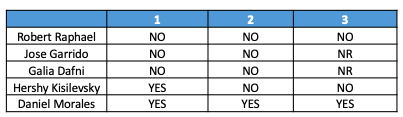
\includegraphics[scale=0.8]{images/table.png}
\caption[Interviewee Answers]{Interviewee Answers. Personal Creation}
\end{figure}


A pie chart was generated to facilitate the analysis of the questions.\\

\begin{figure}[H]
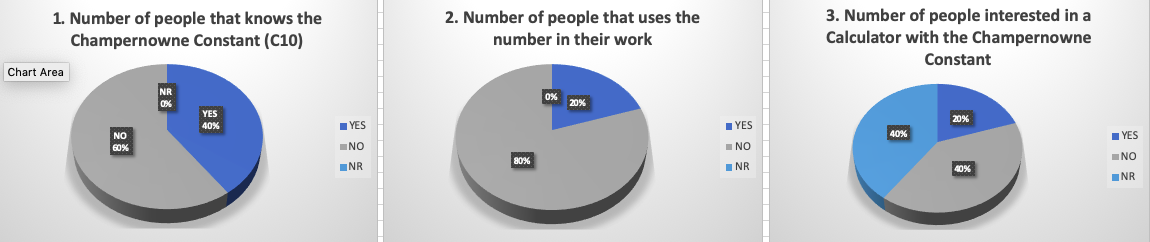
\includegraphics[scale=0.4]{images/pie.png}
\caption[Interviewee Answers Pie Graph]{Interviewee Answers Pie Graph. Personal Creation}
\end{figure}


The Image and Table show that only two of the people know about the number. This is due to the fact that both of them were recommended as an expert by the other potential interviewees. Even though two interviewees knew about the number, one of them does not uses for his work or is interested in a calculator with this number.

From this step is evident that this number is not of common knowledge even for specialist in the Math area, which makes harder to find potential users interested in a calculator.

Additionally, from the interview it is important to mention that even though one of the interviewees would not use a calculator for this number, both of them established important characteristics of the number:
\begin{enumerate}
\item {The classification of the number and its relation to other numbers.}
\item {The multiple ways of representing the number.}
\item {The combination of uses between the multiple bases of the number.}
\item {The fact that it is a constructed number which makes it possible to identify the position of where certain patterns of number occur.}
\item {The fact that it is a normal and transcendental.}
\end{enumerate}
As part of the applications:
\begin{enumerate}
\item {One of the interviewee would not be interested in its use for randomness.}
\item {It is used in cryptography (encoding and decoding messages).}
\item {It generates infinite possible patterns.}
\item {Its behaviour it is important for different fields.}
\end{enumerate}
In relation to the expectations for the calculator, one of the interviews mentioned that he would like if the calculator could recognize patterns and associate them with its translation, like a dictionary. 

Finally, one of the interviews said that he would prefer a calculator that can be accessed online without the need of a computer and the other a calculator that doesn't require internet to work from a Desktop or mobile application.

\section{PROBLEM 3: Persona}

A persona is an archetypical user of a system. It is based on research into real users of a system.  It is a concrete model and it places a human face for the developers.

In this project two personas where created because of the differences between the users. Both of them have experience in Numbers Theory but they have different levels of education and different views of the expected functionalities of the calculator.

The first persona is based on the interview of Daniel Morales and the second persona is based in the interview of professor Hershy Kisilevsky.
%%%%%%%%%%%%%%%%%%%%%%%%%%%%%%%%%%%%%%%%%%%%%%%%%%%%%%%%%%%%%%
\newpage

\subfile{personas/studentpersona}

\newpage
%%%%%%%%%%%%%%%%%%%%%%%%%%%%%%%%%%%%%%%%%%%%%%%%%%%%%%%%%%%%%%
%%%%%%%%%%%%%%%%%%%%%%%%%%%%%%%%%%%%%%%%%%%%%%%%%%%%%%%%%%%%%%

\subfile{personas/professorpersona}

\newpage
%%%%%%%%%%%%%%%%%%%%%%%%%%%%%%%%%%%%%%%%%%%%%%%%%%%%%%%%%%%%%%
\section{PROBLEM 4: Domain Model}

\subsection{Description}

The domain model is vocabulary, with respect to some goal, of a domain [11]. For this project all the important concepts are represented in the domain. Even though the mathematical expression in this calculator is going to be represented only by one number, its existence is necessary so it is not represented as an abstract element. Additionally, details are provided for all the components of an expression since they are relevant for some of the methods to calculate the number (the series for different bases).

\subsection{Concepts}

\begin{enumerate}
\item Calculator: it is an electronic device used for doing mathematical processes such as adding, subtracting, dividing, and multiplying numbers[12]. In this project the calculator will be a system that provides numeric and graphical operations. \newline

\item Mathematical Expression: it is a finite combination of symbols formed according to rules that depend on the context. Mathematical symbols can be numbers (constants), variables, operations, functions, brackets, punctuation, and grouping to help determine order of operations, and other aspects of logical syntax [13]. In the calculator the purpose is that the mathematical expression to be calculated is formed only by the value of the number. \newline

\item Operand: An operand is an object of a mathematical or other operation. These are commonly expressed in computer programming as constants or variables [14]. A constant in this project is represented by a number. \newline

\item Operator: it is any symbol that indicates an operation to be performed. Examples are addition "+" and subtraction "-". An operator may be regarded as a function, transformation, or map, in the sense that it associates or “maps” elements from one set to elements from another set [15]. Operators are different to functions since they receive a determined number of parameters (they usually are unary or binary). \newline

\item Number:a sign or symbol representing a unit that forms part of the system of counting and calculating[16]. It is consider a constant because its value doesn't change. \newline

\item Irrational Algebraic Number: an algebraic number is any real or complex number that is a solution of an algebraic equation [17]. Algebraic numbers can be rational or irrational. \newline

\item Transcendental Number: is a real number or complex number that is not an algebraic number, not a root of a nonzero polynomial equation with integer coefficients [18]. \newline

\item Rational Number: it is any number that can be expressed as the quotient or fraction p/q of two integers, a numerator p and a non-zero denominator q [19]. \newline

\item Irrational Number: it is any real number that is not rational, and its decimal expression is not exact or periodic [20]. \newline

\item Variable: A variable is a symbol on whose value a function, polynomial, etc., depends [21]. It represented by a letter. \newline

\item Function: is a relation that uniquely associates members of one set with members of another set [22]. They are relevant as part of the expression but are not going to be used as part of the calculator.\newline

\item Special Operation:  in this project represents an operation that was suggested as an application of the number by one of the users. \newline

\item Find Numeric Pattern: this is one of the specific applications of the number. Since any normal number contains in their decimal expression any possible pattern the user will provided the pattern and the calculator will give the position of its occurrence. \newline

\item Message Encryption: it is known that the decimal expansion of any transcendental number is non-terminating. The mountain of the number are its decimals. The mountain is used in the encryption of messages by using the the position of a decimal place of the number as key and replacing all the elements in the message by the values in the result of the position mod 26 [23]. \newline

\item Message Decryption: for decryption it is necessary indicate the number that in the case of our calculator is the Champernowne Constant, and indicate the position of the decimal expansion, where the encryption process has begun [23]. \newline

\item User: is a person who interacts with the software system [24].\newline

\item Cryptography: it is the practice of creating and understanding codes that keep information secret [25]. \newline

\end{enumerate}

\subsection{Relationships}

\begin{enumerate}
\item Mathematical Expression Aggregations: a mathematical expression is composed by multiple elements, but when it is deleted its components are still relevant and they are used for special operations.\newline

\item Operand Generalization: There are two types of operands and the decomposition of number is shown until its last elements to demonstrate the existence of transcendental numbers since the Champernowne Constant is transcendental.\newline

\item Message Encryption Aggregation: this is shown as an aggregation since message encryption existed even before the term cryptography was created.

\item Special Operation Generalization: it specifies the two possible applications of the number described by the interviewees.\newline

\item Is-Calculated Association: is an association between the calculator and the mathematical expression. The mathematical expression is the number for this calculator and its value most be determined.\newline

\item Introduces Association: it is an association between the user and the mathematical expression. The user have to provide the expression to be calculated.\newline

\item Executes Association: it is a relation between the user and the special operations, this exists since the user can applied this operations to the number.\newline

\item Perform Association: it is a relation between the calculator and the special operations that are performed by it.\newline

\item Used-To-Find-Repetition Association: this association describes the role of the number, the find pattern operation search for a repeated pattern in its decimals.\newline

\item Use-For-Ciphering Association: a substitution cipher is a method of encrypting by which letters are replaced with ciphertext following an specific system. The number would provide the necessary elements to determine this system and perform the encryption.\newline

\item Use-For-Deciphering Association: this association reverse indicates the reverse of the Ciphering process, the number and a key are used by the user to obtain the original message.\newline

\end{enumerate}

\subsection{Domain Model}

\begin{figure}[h]
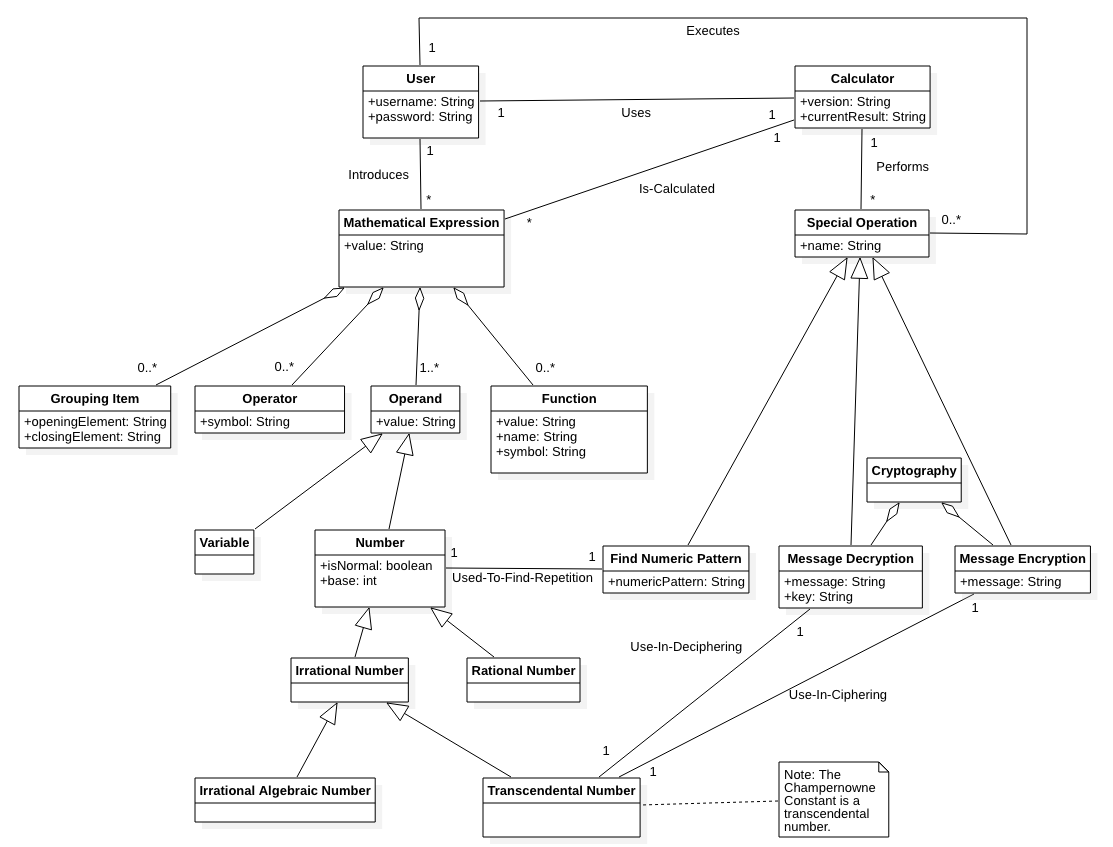
\includegraphics[scale=0.46]{images/DomainModel.png}
\caption[Domain Model]{Domain Model. Personal Creation}
\end{figure}

%%%%%%%%%%%%%%%%%%%%%%%%%%%%%%%%%%%%%%%%%%%%%%%%%%%%%%%%%%%%%%
\section{PROBLEM 5: Use Case Model}

\subsection{Use Case Model Diagram}

\begin{figure}[H]
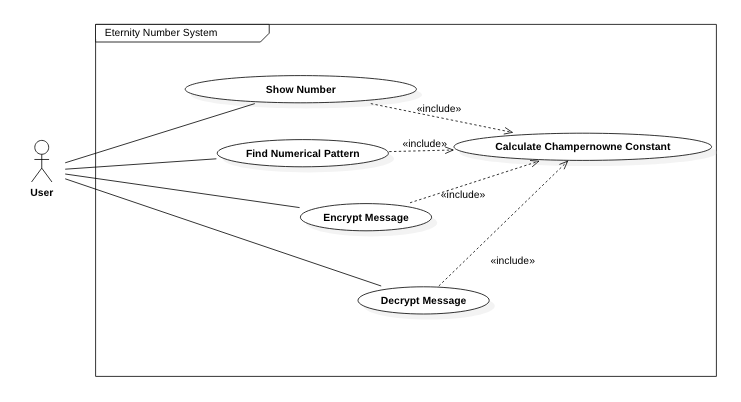
\includegraphics[scale=1.1]{images/useCaseDiagram.png}
\caption[Use Case Diagram]{Use Case Diagram. Personal Creation}
\end{figure}
\subsection{Activity Diagram}

\begin{figure}[H]
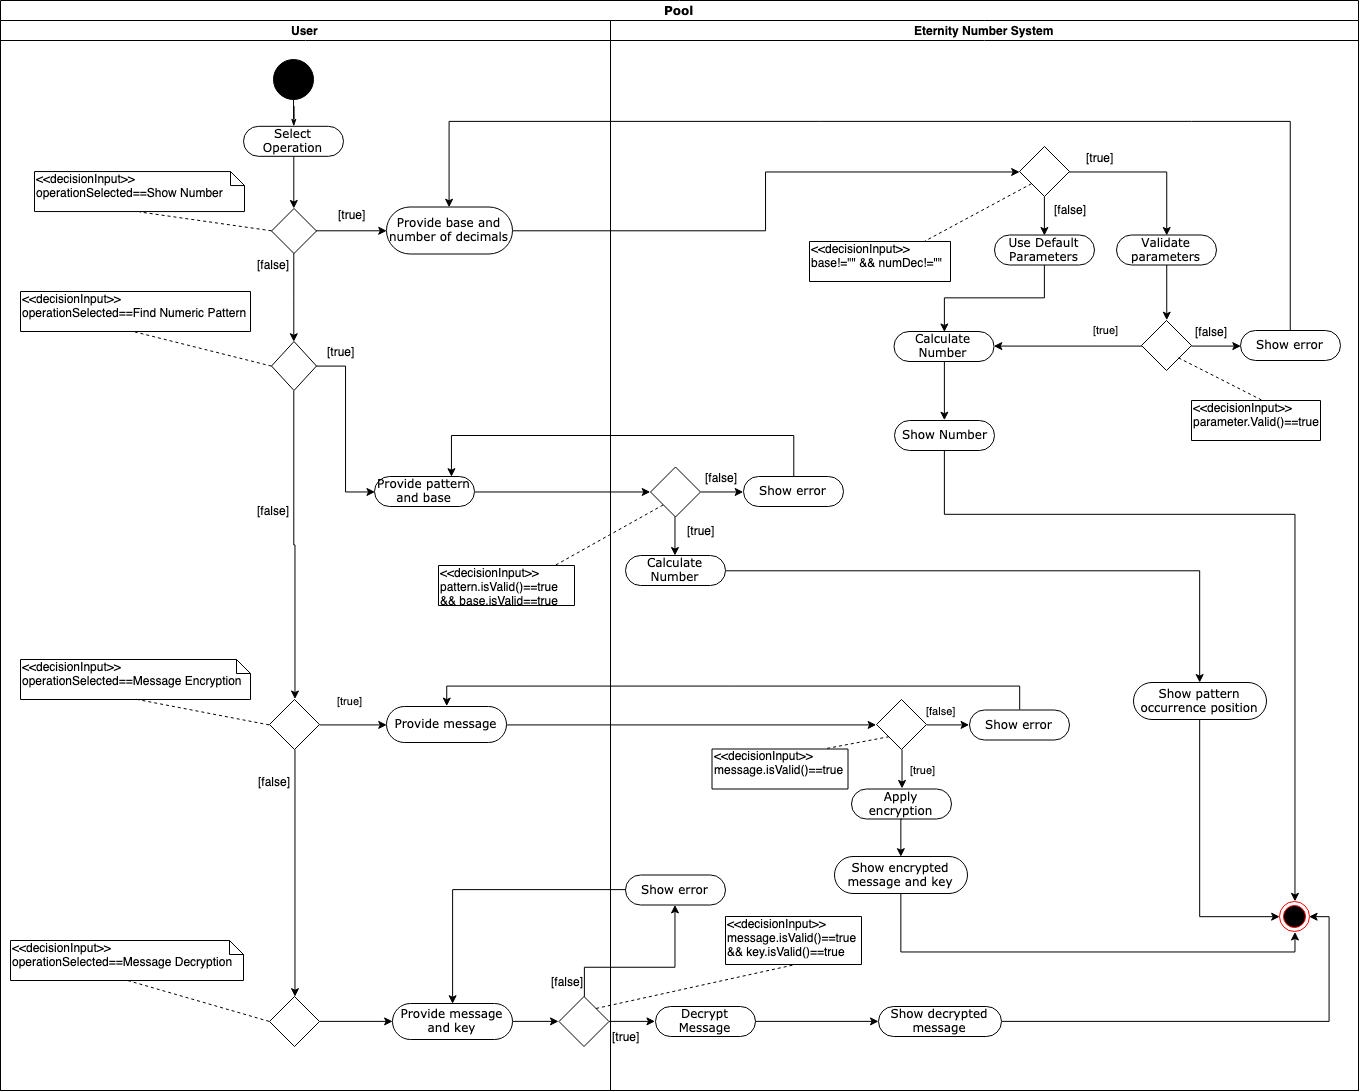
\includegraphics[scale=0.35]{images/activity.png}
\caption[Activity Diagram]{Activity Diagram. Personal Creation}
\end{figure}

\subsection{Use Cases - Normal Scenario}

Even though the calculation of the Champernowne Constant is important for all the use cases, it is only performed by the system and it doesn't require user interaction. 

\subsubsection{UC-1 Show Number}

ID: UC-1

Description: The user requires to display the number to the user.

Pre-Condition: The user download the application
Post-Condition: N/A

Trigger: The clients select show number option.

Actors: User, EternityNumberSystem

\textbf Normal Scenario:
\begin{enumerate}
\item User\#1 selects show Champernowne Constant.
\item The System calculates the number.
\item The System shows the number.
\newline
\end{enumerate}

\begin{figure}[H]
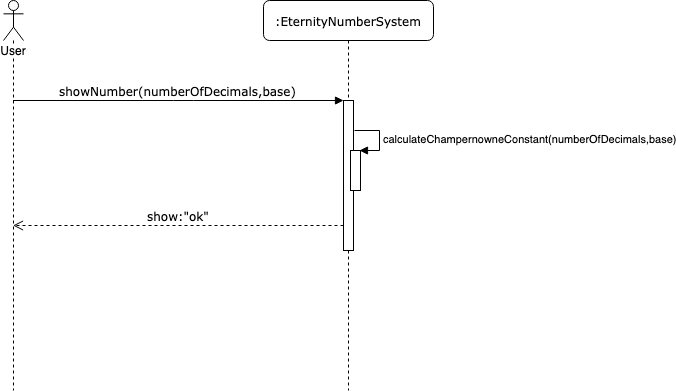
\includegraphics[scale=0.75]{images/showNumber.png}
\caption[UC-1 Show Number]{UC-1 Show Number. Personal Creation}
\end{figure}

\subsubsection{UC-2 Find Numeric Pattern}

ID: UC-2

Description: the user provides a numeric pattern and the system shows the position of occurrence of this pattern in the decimals of the number.

Pre-Condition: The user download the application
Post-Condition: N/A
Trigger: The clients select Find Numeric pattern option.

Actors: User, EternityNumberSystem

\textbf Normal Scenario:
\begin{enumerate}
\item User\#1 selects find numeric pattern.
\item The User\#1 provides the pattern and the base to use to calculate the Champernowne Constant.
\item The System calculates the number.
\item The System finds the pattern.
\item The System shows the position of occurrence.
\newline
\end{enumerate}

\begin{figure}[H]
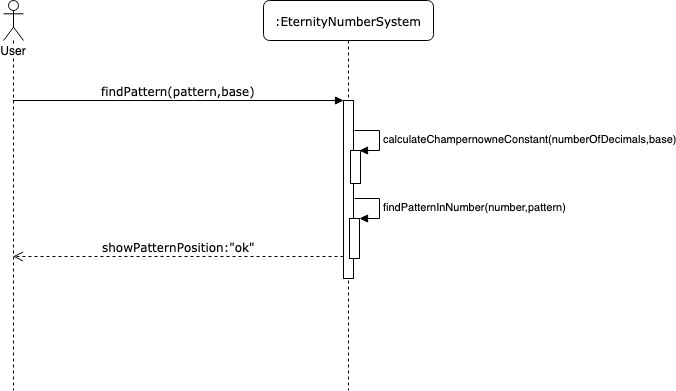
\includegraphics[scale=0.75]{images/findPattern.png}
\caption[UC-2 Find Numeric Pattern]{UC-2 Find Numeric Pattern. Personal Creation}
\end{figure}

\subsubsection{UC-3 Encrypt Message}

ID: UC-3

Description: The user requires to encrypt a message using the mountain of the Champernowne Constant. The system will take a decimal position and return the encrypted message with a key.

Pre-Condition: The user download the application
Post-Condition: N/A

Trigger: The clients select Encrypt Message operation.

Actors: User, EternityNumberSystem

\textbf Normal Scenario:
\begin{enumerate}
\item User\#1 selects Encrypt Message operation.
\item User\#1 provides the message to be encrypted.
\item The System calculates the number.
\item The System encrypt the message based on the number.
\item The system shows the encrypted message and the key.
\newline
\end{enumerate}

\begin{figure}[H]
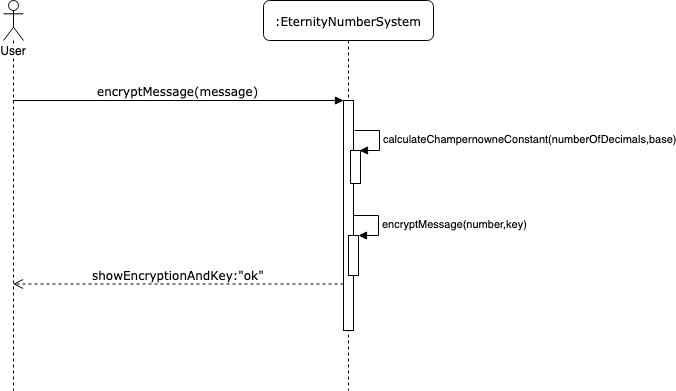
\includegraphics[scale=0.75]{images/MessageEncryption.png}
\caption[UC-3 Message Encryption]{UC-3 Message Encryption. Personal Creation}
\end{figure}

\subsubsection{UC-4 Decrypt Message}

ID: UC-4

Description: The user gives a message and a key to decrypt it using the Champernowne Constant as base. 

Pre-Condition: The user download the application
Post-Condition: N/A

Trigger: The clients select Decrypt Message operation.

Actors: User, EternityNumberSystem

\textbf Normal Scenario:
\begin{enumerate}
\item User\#1 selects Decrypt Message operation.
\item User\#1 provides the message and the key.
\item The System calculates the number
\item The System decrypts the message based on the number.
\item The system shows the decrypted message.
\newline
\end{enumerate}

\begin{figure}[H]
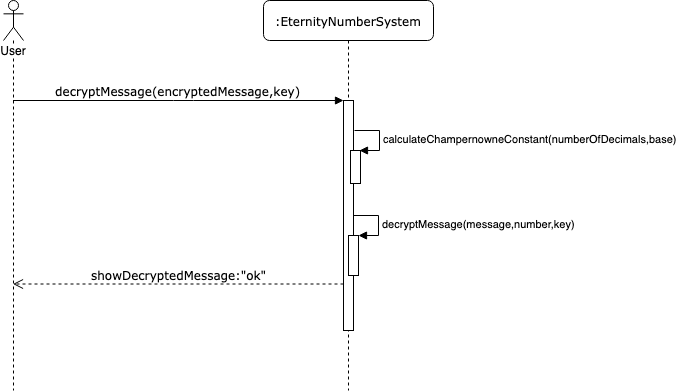
\includegraphics[scale=0.75]{images/messageDecryption.png}
\caption[UC-4 Message Decryption]{UC-4 Message Decryption. Personal Creation}
\end{figure}
%%%%%%%%%%%%%%%%%%%%%%%%%%%%%%%%%%%%%%%%%%%%%%%%%%%%%%%%%%%%%%
\chapter{Conclusion}

The objectives in each problem were achieved, even though the Champernowne Constant is not known for a lot people. The problems allowed to gather different requirements for potential users, gain understanding about the applications and characteristics of the Champernowne Constant, and catch a glimpse of the functionalities that the calculator should have.

It is important to mention that the operation of the calculator are specifically related with the characteristics of the number. The find pattern is possible since the Champernowne Constant is a normal number, and the cryptography features are based on the fact that it is a transcendental number.

This report shows and intermediate view of the functionalities of the system; however, more problems are require before the implementation of the calculator. This project only shows an initial state of the development process.

\newpage
\begin{thebibliography}{9}

\bibitem{website} 
Champernowne Constant. (2019). Retrieved from: \\\texttt{http://oeis.org/search?q=Champernowne+constant\&sort=\&language=\&go=Search}

\bibitem{bib} 
D.G. Champernowne, The Construction of Decimals Normal in the Scale of Ten, J. London Math. Soc. 8, 1933, p. 254-260.
 
\bibitem{bib1} 
K. Mahler, Arithmetische Eigenschaften einer Klasse von Dezimalbrüchen, Proc. Konin. Neder. Akad. Wet. Ser. A. 40, 1937, p. 421-428.
 

\bibitem{website1} 
Transcendental Number. (2019). Retrieved from:  \\\texttt{http://mathworld.wolfram.com/TranscendentalNumber.html}

\bibitem{bib2} 
H. Von Baeyer, Information: The New Language of Science, Weidenfeld and Nicolson, Great Britain, 2003, p. 101-102, 104, 123-124. 

\bibitem{website2} 
Champernowne Constant. (2019). Retrieved from:  \\\texttt{http://www.infiniteabyss.org/2010/02/11/an\_interesting\_property\_of\_champernownes\_number.html}

\bibitem{website3} 
Champernowne Constant cfe Coefficient Calculation. (2019). Retrieved from: \\\texttt{http://code.google.com/p/champernowne-constant-cfe-coefficient-calculationhwm/downloads/list find\_num\_pos.rb}

\bibitem{website4} 
On the High Water Mark Convergents of Champernowne’s Constant in Base Ten. (2019). Retrieved from: \\\texttt{https://arxiv.org/pdf/1210.1263.pdf}

\bibitem{website5} 
AN INTERESTING PROPERTY OF CHAMPERNOWNE'S NUMBER.  (2019). Retrieved from: \\\texttt{https://www.kanonical.io/an\_interesting\_property\_of\_champernownes\_number/}

\bibitem{website6} 
P. Kantham. INTRODUCTION TO INTERVIEWS.(2019). Retrieve from:
\\\texttt{https://users.encs.concordia.ca/\~kamthan/courses/soen-6481/interviews\_introduction.pdf}

\bibitem{website13}
P. Kantham. INTRODUCTION TO DOMAIN MODELING. (2019). Retrieve from:
\\\texttt{https://users.encs.concordia.ca/\~kamthan/courses/soen-6481/domain\_modeling\_introduction.pdf}

\bibitem{website7}
Calculator.(2019).Cambridge Dictionary. Retrieve from: \\\texttt{https://dictionary.cambridge.org/es/diccionario/ingles/calculator}

\bibitem{bib3}
Redden, John. Elementary Algebra. Flat World Knowledge, 2011.

\bibitem{website8}
Operand.(2019).Techopedia. Retrieve from: \\\texttt{https://www.techopedia.com/definition/3483/operand}

\bibitem{website16}
Operator.Encyclopedia Britanica.(2019).Retrieve from: \\\texttt{https://www.britannica.com/topic/operator}

\bibitem{website9}
Number.(2019).Cambridge Dictionary. Retrieve from: \\\texttt{https://dictionary.cambridge.org/es/diccionario/ingles/number}

\bibitem{bib4}
Birkhoff \& Mc Lane. Álgebra Moderna. Algebraic Numbers.

\bibitem{website10}
Weisstein, Eric W. Transcendental Number. (2019).Retrieve from: \\\texttt{http://mathworld.wolfram.com/}

\bibitem{bib5}
Arias Cabezas, Jose Maria; Maza Saez, Ildefonso (2008). «Aritmetica y Algebra». En Carmona Rodriguez, Manuel; Diaz Fernandez, Francisco Javier. Matematicas 1. Madrid: Grupo Editorial Bruño, Sociedad Limitada. p. 14.

\bibitem{bib6}
Rosen, Kenneth. Discrete Mathematics and its Applications (6th ed.). New York, NY: McGraw-Hill. pp. 105, 158–160.

\bibitem{website11}
Variable. Wolfram Math World. (2019).Retrieve from: \\\texttt{http://mathworld.wolfram.com/Variable.html}

\bibitem{website12}
Function. Wolfram Math World. (2019).Retrieve from: \\\texttt{http://mathworld.wolfram.com/Function.html}

\bibitem{website15}
M. K. Viswanath. Transcendental Numbers and Cryptography. (2014). Retrieve from: \\\texttt{http://www.m-hikari.com/ams/ams-2014/ams-173-176-2014/viswanathAMS173-176-2014.pdf}

\bibitem{website14}
P. Kantham. INTRODUCTION TO USER MODELING. (2019). Retrieve from:
\\\texttt{https://users.encs.concordia.ca/\~kamthan/courses/soen-6481/user\_modeling\_introduction.pdf}

\bibitem{website17}
Criptography.(2019).Cambridge Dictionary. Retrieve from: \\\texttt{https://dictionary.cambridge.org/es/diccionario/ingles/cryptography}

\end{thebibliography}

\end{document}
